\title{Laboratory 1 - Fluids Labs}
\author{
        Sergio M. Vanegas A.\\
                Department of Mathematics\\
        Polimi---Politecnico di Milano\\
        Milano, Italia
}
\date{\today}

\documentclass[12pt]{article}

\usepackage{amsmath}
\usepackage{graphicx}

\begin{document}
\maketitle

\begin{abstract} 
        The first test case is the steady-state development of incompressible flow between two parallel plates in the laminar regime (Figure~\\\ref{fig:sketch}). The plates are considered infinite in the direction transversal to the flow. The flow develops from a condition of uniform velocity (rectangular profile) imposed at the inlet boundary, reaching a fully-developed state at a certain distance downstream of it. \cite{FL:01}
\end{abstract}

\section{Introduction}
        The fully developed laminar flow between two parallel plates admits an analytical solution (plane Poiseuille flow):

        \begin{equation}
                \begin{cases}
                        u(x,y,z) = u(y) = - \frac{\delta ^ 2}{2 \mu} \frac{dp_e}{dx} \frac{y}{\delta} (2 - \frac{y}{\delta}) \; v(x,y,z) = 0 \; w(x,y,z) = 0 \\
                        \frac{dp_e}{dx} = const < 0 \\
                        \tau_{yx}(x,y,z) = - 2 \mu \frac{1}{2} \left( \frac{\partial u}{\partial y} + \frac{\partial v}{\partial x} \right) = - \mu \frac{du}{dy} = \frac{dp_e}{dx} (\delta - y) = \tau_{yx}(y)
                \end{cases}
        \end{equation}

        Where \( \mu \) is the dynamic viscosity of the fluid, \( \delta \) is the half-distance between the plates, \(u, v, w\) are the velocity components along directions \( x, y, z \) (Figure~\ref{fig:sketch}), \( p_e \) is the excess pressure with respect to the hydrostatic component, and \( \tau_{yx} \) is the only nonzero shear stress. \cite{FL:01}

        \begin{figure}[!ht]
                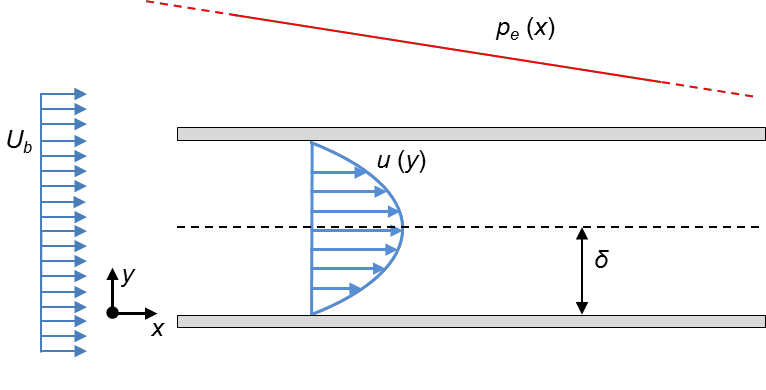
\includegraphics[width=0.7\textwidth]{Case_Sketch.png}
                \centering
                \caption{Sketch of the Case}
                \label{fig:sketch}
        \end{figure}

        The configuration of the problem is as follows:
        \begin{itemize}
                \item Length \( L,\, L_p \) to be defined,
                \item Half-channel height \(\delta = 5 \; mm\),
                \item Bulk velocity \( U_b = 5 \; mm/s \),
                \item Fluid: Water at \( 20^{\circ}C \;\; ( \rho = 998.23 \; kg/m^3\), \\ Kinematic Viscosity \( \nu = 1.006E-6 \; m^2/s ) \).
        \end{itemize}

        \begin{figure}[!ht]
                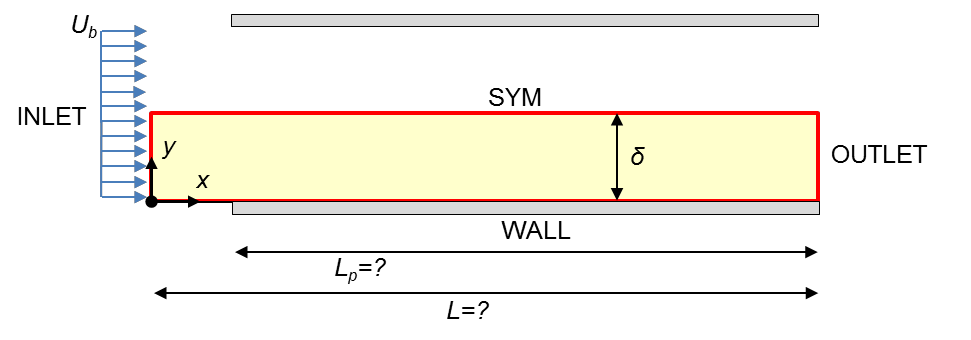
\includegraphics[width=0.7\textwidth]{Conditions.png}
                \centering
                \caption{Domain and boundary conditions}
                \label{fig:conditions}
        \end{figure}

        \paragraph{Outline}
        The remainder of the report is organizedas follows: Section~\ref{sec:developed_flow} provides some gross estimate of the required \( L_p \) to achieve a fully-developed flow in terms of channel height; Section~\ref{sec:independence} shows how a suitable configuration of the cartesian computational mesh was found; Section~\ref{sec:CFD_validation} compares the simulated solution with the analytical model both graphically and numerically; Finally, Section~\ref{sec:vorticity} provides some analysis regarding the vorticity profile on both the developing and fully-developed region.

\section{Fully-developed flow conditions} \label{sec:developed_flow}

\section{Grid independence study} \label{sec:independence}

\section{CFD solution validation} \label{sec:CFD_validation}

\section{Vorticity} \label{sec:vorticity}

\bibliographystyle{abbrv}
\bibliography{main}

\end{document}